\documentclass[a4paper]{article}
\usepackage[warn]{mathtext}
\usepackage[utf8]{inputenc}
\usepackage[T2A]{fontenc}
\usepackage[english,russian]{babel}
\usepackage{indentfirst}
\usepackage{misccorr}
\usepackage{subcaption}
\captionsetup{compatibility=false}
\usepackage{geometry}
\geometry{verbose,a4paper,tmargin=2cm,bmargin=2cm,lmargin=1.5cm,rmargin=1.5cm}
\usepackage{graphicx}
\usepackage{wrapfig}
\usepackage{amsmath}
\usepackage{fancyhdr}
\usepackage{floatflt}
\usepackage{float}
\usepackage{amssymb}
\usepackage{color}
\usepackage{lscape}
\usepackage{hvfloat}
\usepackage{amsfonts}
\usepackage{euscript}
\usepackage{newunicodechar}
\usepackage{booktabs}

\begin{document}
\newcommand{\apple}{\char"F8FF}



\begin{titlepage}
    \vspace*{4cm}
	\centering
    {\scshape\LARGE Московский физико-технический институт\par}
	\vspace{1cm}
	{\scshape\Large Лабораторная работа по общей физике № 4.2\par}
	\vspace{1cm}
    {\huge\bfseries  Исследование энергетического спектра $\beta$-частиц и определение их 
    максимальной энергии при помощи магнитного спектрометра \par}
	\vspace{2cm}
	\vfill
\begin{flushright}
	{\large Выполнила студентка Б01-907}\par
	\vspace{0.3cm}
	{\LARGE Юлия Прохорова}
\end{flushright}
	
	\vfill
Долгопрудный, 2021
% Bottom of the page
\end{titlepage}

\pagestyle{fancy} 
\fancyhead[L]{№ 4.2}
\fancyhead[R]{Юля Прохорова, Б01-907}
\fancyhead[C]{}
\fancyfoot[C]{ \noindent\rule{\textwidth}{0.4pt} \thepage }

\tableofcontents

\newpage


\section{Цель работы}

С помощью магнитного спектрометра исследовать энергетический спектр $\beta$-частиц при распаде
ядер $^{137}Cs$ и определение их максимальной энергии.

\section{Оборудование}
Магнитный спектрометр с короткой линзой, высоковольтный и низковольтный выпрямители, форвакуумный насос и вакууметр, ЭВМ.

\section{Теория}

\textbf{Бета-распадом} называется самопроизвольное превращение ядер, при котором их массовое
число не меняется, а заряд увеличивается или уменьшается на единицу. В нашем случае имеем дело 
с электронным распадом:
$${_Z^A}X \rightarrow {_{Z+1}^A}X + e^- + \tilde{\nu}$$

Освобождающаяся энергия делится между электроном и антинейтрино, дочернему ядру достается очень мало.

Вид спектра $\beta$-частиц показан на рис.\ref{p1}. $W(p_e)dp_e$ - вероятность того, что $\beta$-частица получит импульс в интервале $(p_e, \; p_e+dp_e)$.

\begin{wrapfigure}[17]{l}{145pt}
    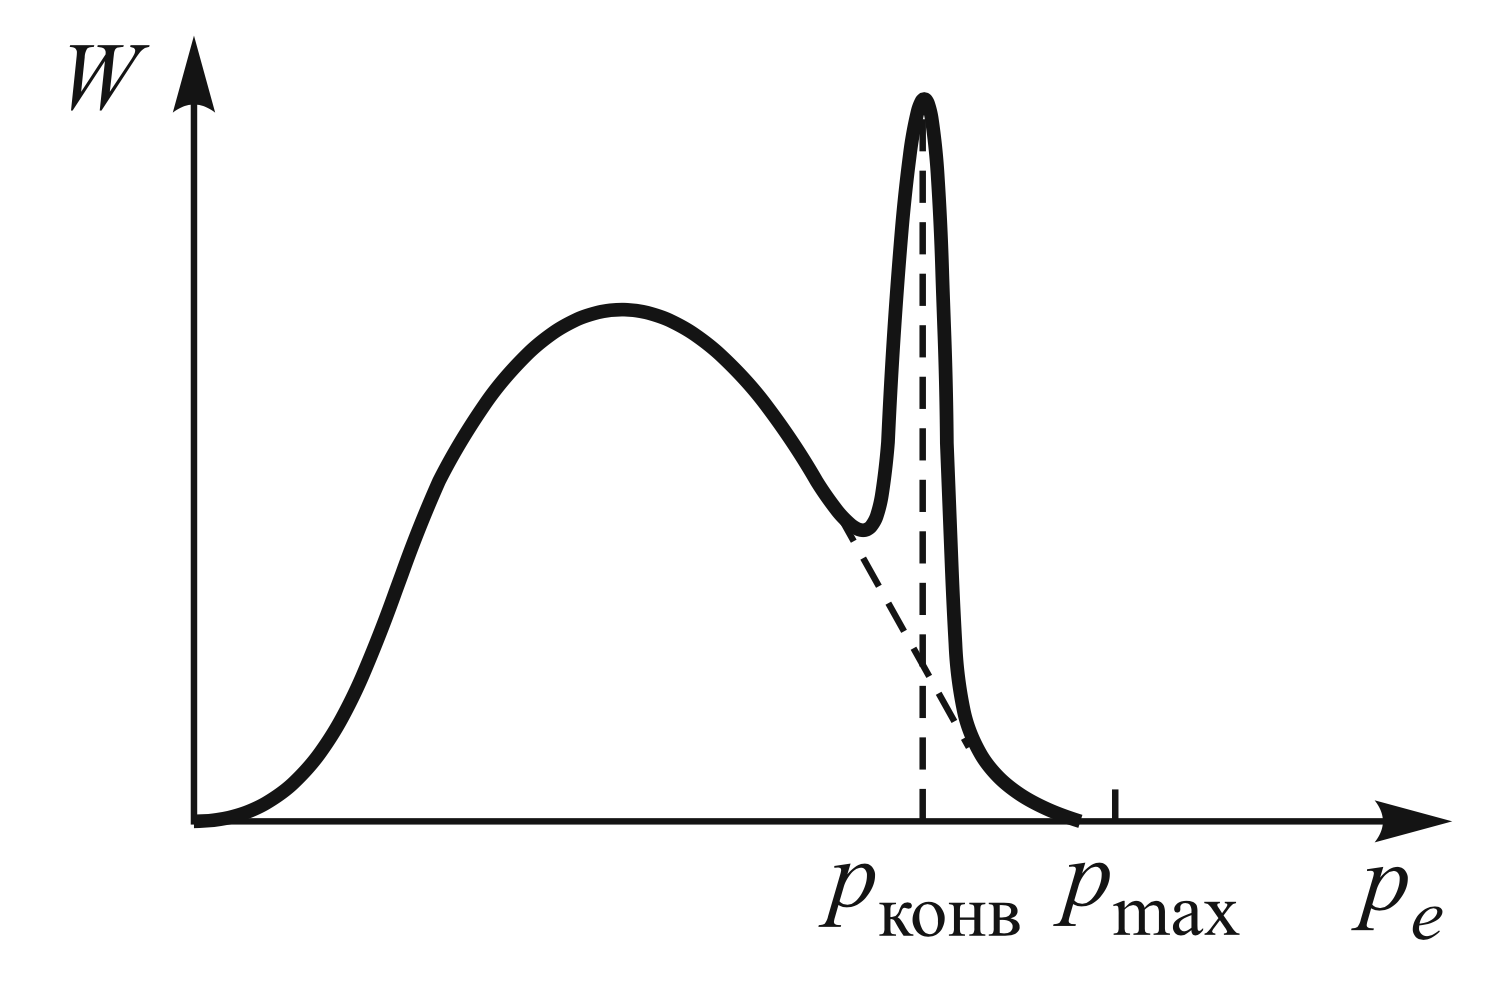
\includegraphics[scale = 0.2]{p1.png}
    \caption{Форма спектра $\beta$-частиц при разрешенных переходах}
    \label{p1}
\end{wrapfigure}

Вероятность $\beta$-распада пропорциональна фазовому объему в векторном пространстве имупульсов
электронов и антинейтрино. Интервалу $(p_e, \; p_e+dp_e)$ соответсввет шаровой слой объема 
$4\pi p_e^2 dp_e$. В пространстве импульсов, уносимых антинейтрино, выделятеся шаровой слой 
площадью $4 \pi p_{\nu}^2$, значит:

\begin{equation}
    W(p_e) dp_e \propto p_e^2 p_{\nu}^2 dp_e 
    \label{eq1}
\end{equation}

Выразим в этом соотношении $p_{\nu}$ через $p_e$. Масса антинейтрино равна нулю, значит:

\begin{equation}
    p_{\nu} = E_{\nu} / c = (T_{max} - T_e)/c
    \label{eq2}
\end{equation}

$E_{\nu}$ - кинетическая энергия антинейтрино, $T_{max}$ - масимально возможная кнетическая энергия
электрона. $T_e$ - фактическая энергия электрона. Подставляя \ref{eq2} в \ref{eq1} получим:

\begin{equation}
    W(p_e)dp_e \propto p_e^2 (T_{max} - T_e)^2 dp_e
    \label{eq3}
\end{equation}

Кинетическая энергия электрона и его импульс связаны:

\begin{equation}
    T_e = \sqrt{p_e^2 c^2 + m_e^2 c^4} - m_e c^2
    \label{eq4}
\end{equation}

Отсюда:

\begin{equation}
    T_{max} - T_e = c (\sqrt{p_{max}^2 + m_e^2 c^2} - \sqrt{p_e^2 + m_e^2 c^2})
    \label{eq5}
\end{equation}

Уравнение (\ref{eq5}) описывает спектр как широкий колокол (рис.\ref{p1}) 

Дочерние ядра нередко бывают возбужденными, поэтому они могут излучать $\gamma$-квант или 
передавать избыток электрону на внутренней оболочке. Такие излучаемые электроны называются 
\textbf{конверсионными}. На спектре  (рис.\ref{p1}) видна монохроматическая линия, ширина
которой обусловлена лишь разрешающей способностью спектрометра.

\section{Экспериментальная установка}

Энергию частиц определяют с помощью $\beta$-спектрометра. В работе используется 
магнитный спеткрометр с "короткой линзой", сцинтиллятором и ФЭУ. По расчету, 
тонкая катушка эквивалент на линзе:

\begin{equation}
    \frac{1}{f} \varpropto \frac{I^2}{p_e^2}
    \label{eq6}
\end{equation}

\begin{figure}[h]
	\begin{center}
	\begin{minipage}[h]{0.45\linewidth}
	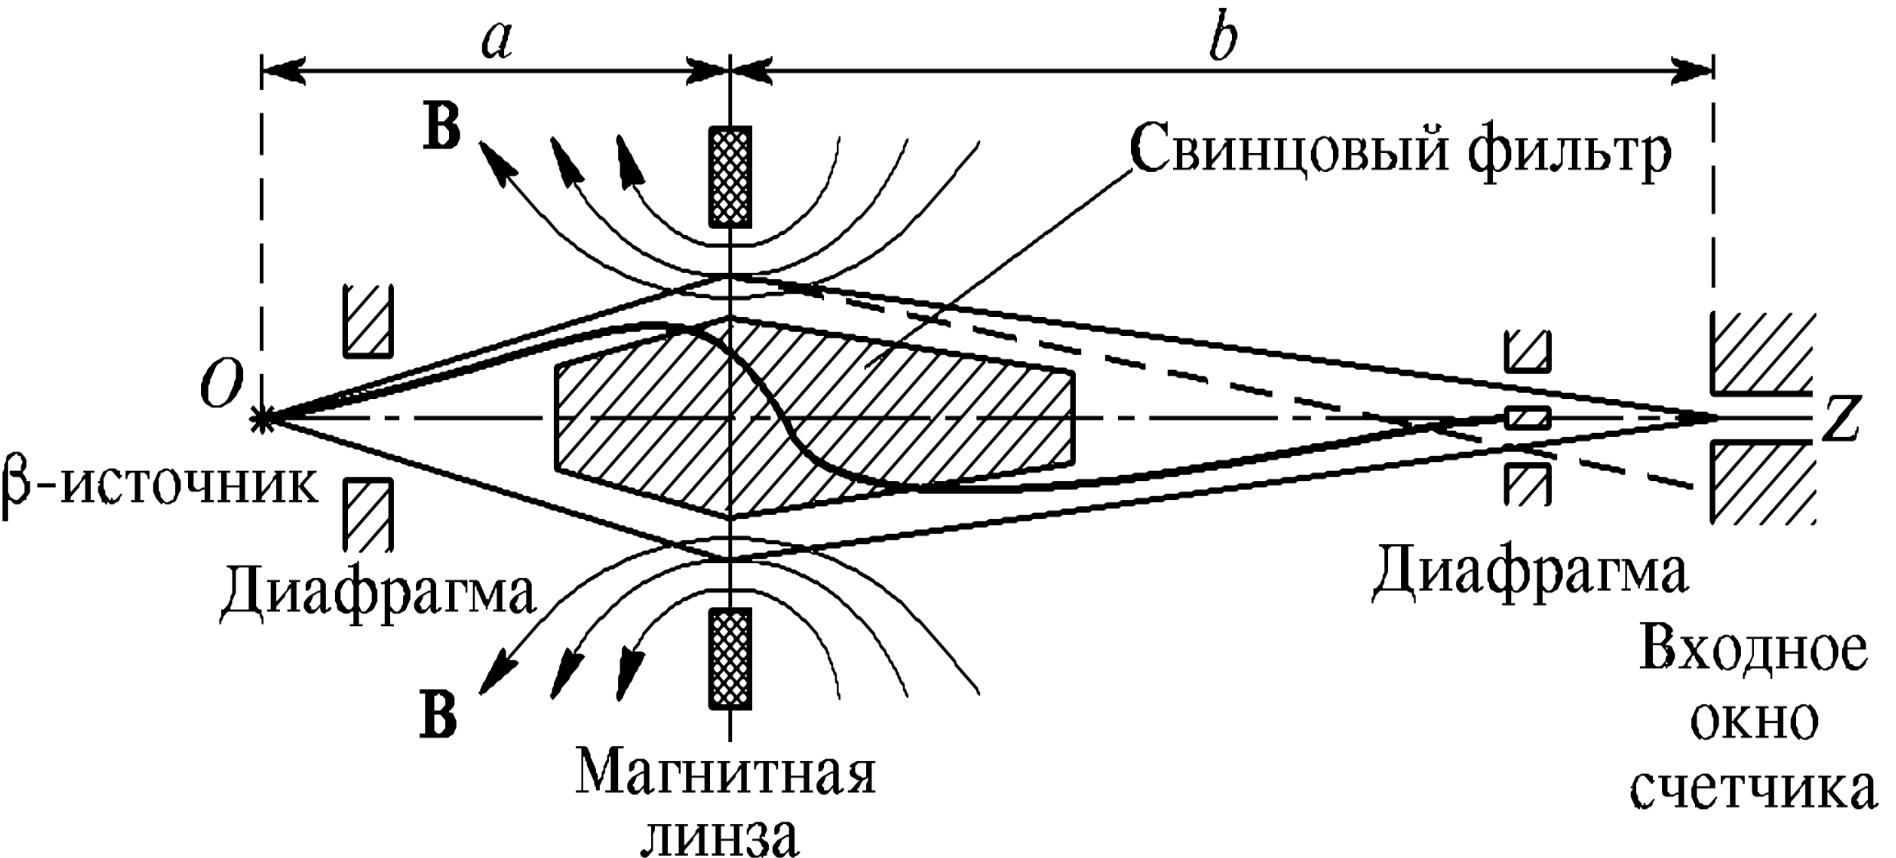
\includegraphics[width=1\linewidth]{p2.png}
	\caption{Схема $\beta$-спектрометра с короткой магнитной линзой} 
    \label{p2}
	\end{minipage}
	\hfill 
	\begin{minipage}[h]{0.45\linewidth}
	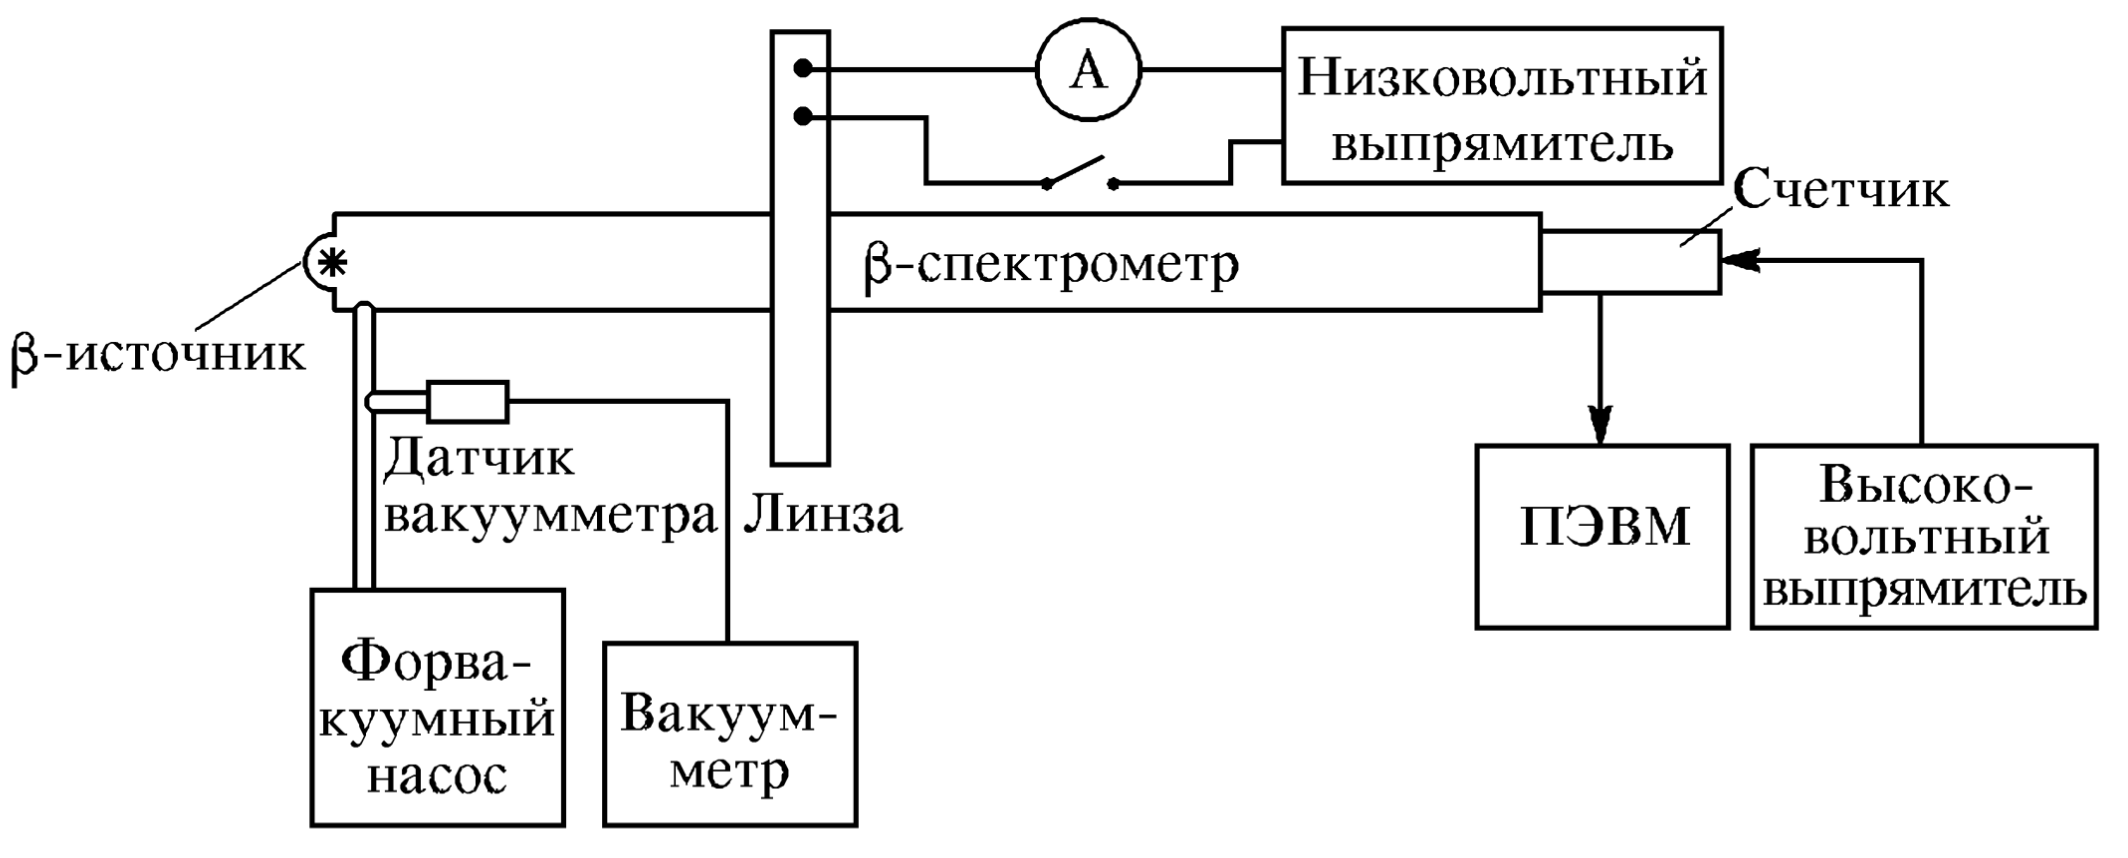
\includegraphics[width=1\linewidth]{p3.png}
	\caption{Блок-схема измерительного комлпекса}
	\label{p3}
	\end{minipage}
	\end{center}
\end{figure}

При заданной силе тоув на входное окно счетчика фокусируются электоны с 
определенным значением импульса. Импульс сфокусированнх электонов пропорционален 
величине тока I:

\begin{equation}
    p_e = k\cdot I
    \label{eq7}
\end{equation}

Константа прибора k определяется по известной конверсионной линии.

Линза обладает абберацией, поэтому установлены кольцевые диафрагмы, ограничивающие
углы вылетов электронов. Также установлен свинцовый фильтр, сдерживающий $\gamma$-кванты 
и электроны, летящие прямо. Величина $\Delta p_e$ - разрешающая способность.

Рассмотрим связь между числом частиц, регистрируемых установкой, и функцией $W(p_e)$, 
определяемой формулой (\ref{eq3}):

\begin{equation}
    N(p_e) \approx W(p_e) \Delta p_e 
    \label{eq8}
\end{equation}

Фокус линзы зависит от импульса, частицы проходят мимо при больших $\Delta f$, 
продиффиренцируем (\ref{eq6})

\begin{equation}
    \Delta p_e = \frac{1}{2} \frac{\Delta f}{f} p_e
    \label{eq9}
\end{equation}

Таким образом, ширина интервала $\Delta p_e$ пропорциональна импульсу. Подставим 
(\ref{eq9}) в (\ref{eq8}):

\begin{equation}
    N(p_e) = C \cdot W(p_e) p_e
    \label{eq10}
\end{equation}

где С - некоторая константа.

Давление в спектрометре поддерживается на уровне 0.1 Торр и измеряется вакууметром.
Откачка освществляется форвакуумным насосом. Высокое напряжение на ФЭУ подается
от стабилизированного выпрямителя.


\section{Ход работы}

\begin{enumerate}
    \item Включаем пересчетный прибор, высоковольтный выпрямитель и вакууметр. Откачиваем давление форвакуумным насосом.
    \item Включаем рабочее напряжение на ФЭУ.
    \item Убеждаемся, что спектрометр корректно работает, для этого увеличиваем ток в катушке, мы должны наблюдать силный рост счетов с повышением тока.
    \item Проведем измерения в интервале от 0.1 до 3.7А с шагом 0.1А, каждое измерение длительностью $t = 100с$.
    \item Измерим фоновый счет спектрометра при отсутствующем и максимальном токе в линзе. Составим линейную зависимость.
    \item Занесем данные в таблицу \ref{t1} и произведем необходимые рассчеты.

\begin{center}
    \begin{table}[H]
\centering
\caption{Данные}
\label{t1}
\begin{tabular}{rrrrrrr}
\toprule
 № &  I, A &  N, 1/c &  Nf(I) &  N-Nf, 1/c &  p\_e, кэВ/c &  T\_e, кэВ \\
\midrule
 1 & 0.100 &   1.410 &  1.344 &      0.066 &      31.672 &     0.982 \\
 2 & 0.200 &   1.230 &  1.329 &     -0.099 &      63.344 &     3.919 \\
 3 & 0.300 &   1.540 &  1.313 &      0.227 &      95.016 &     8.775 \\
 4 & 0.400 &   1.510 &  1.298 &      0.212 &     126.688 &    15.499 \\
 5 & 0.500 &   1.560 &  1.282 &      0.278 &     158.359 &    24.020 \\
 6 & 0.600 &   1.799 &  1.266 &      0.533 &     190.031 &    34.254 \\
 7 & 0.700 &   2.079 &  1.251 &      0.828 &     221.703 &    46.105 \\
 8 & 0.800 &   2.509 &  1.235 &      1.274 &     253.375 &    59.472 \\
 9 & 0.900 &   2.879 &  1.220 &      1.659 &     285.047 &    74.253 \\
10 & 1.000 &   3.749 &  1.204 &      2.545 &     316.719 &    90.342 \\
11 & 1.100 &   4.639 &  1.188 &      3.451 &     348.391 &   107.637 \\
12 & 1.200 &   5.558 &  1.173 &      4.385 &     380.062 &   126.040 \\
13 & 1.300 &   6.638 &  1.157 &      5.481 &     411.734 &   145.458 \\
14 & 1.400 &   7.508 &  1.141 &      6.367 &     443.406 &   165.803 \\
15 & 1.500 &   9.087 &  1.126 &      7.961 &     475.078 &   186.993 \\
16 & 1.600 &   9.277 &  1.110 &      8.167 &     506.750 &   208.954 \\
17 & 1.700 &   9.407 &  1.095 &      8.312 &     538.422 &   231.619 \\
18 & 1.800 &  10.597 &  1.079 &      9.518 &     570.094 &   254.923 \\
19 & 1.900 &  10.097 &  1.063 &      9.034 &     601.766 &   278.810 \\
20 & 2.000 &  10.837 &  1.048 &      9.789 &     633.438 &   303.230 \\
21 & 2.100 &  10.297 &  1.032 &      9.265 &     665.109 &   328.135 \\
22 & 2.200 &   9.937 &  1.017 &      8.920 &     696.781 &   353.484 \\
23 & 2.300 &   9.237 &  1.001 &      8.236 &     728.453 &   379.238 \\
24 & 2.400 &   7.258 &  0.985 &      6.273 &     760.125 &   405.363 \\
25 & 2.500 &   6.548 &  0.970 &      5.578 &     791.797 &   431.829 \\
26 & 2.600 &   5.378 &  0.954 &      4.424 &     823.469 &   458.608 \\
27 & 2.700 &   4.039 &  0.939 &      3.100 &     855.141 &   485.673 \\
28 & 2.800 &   3.399 &  0.923 &      2.476 &     886.812 &   513.004 \\
29 & 2.900 &   3.629 &  0.907 &      2.722 &     918.484 &   540.578 \\
30 & 3.000 &   5.458 &  0.892 &      4.566 &     950.156 &   568.377 \\
31 & 3.050 &   7.618 &  0.884 &      6.734 &     965.992 &   582.356 \\
32 & 3.100 &  10.117 &  0.876 &      9.241 &     981.828 &   596.384 \\
33 & 3.150 &  12.676 &  0.868 &     11.808 &     997.664 &   610.461 \\
34 & 3.200 &  14.686 &  0.860 &     13.826 &    1013.500 &   624.585 \\
35 & 3.250 &  14.446 &  0.853 &     13.593 &    1029.336 &   638.753 \\
36 & 3.300 &  12.986 &  0.845 &     12.141 &    1045.172 &   652.964 \\
37 & 3.350 &  10.617 &  0.837 &      9.780 &    1061.008 &   667.216 \\
38 & 3.400 &   8.967 &  0.829 &      8.138 &    1076.844 &   681.508 \\
39 & 3.450 &   6.948 &  0.821 &      6.127 &    1092.680 &   695.839 \\
40 & 3.500 &   4.789 &  0.814 &      3.975 &    1108.516 &   710.208 \\
41 & 3.600 &   2.229 &  0.798 &      1.431 &    1140.188 &   739.051 \\
42 & 3.700 &   1.510 &  0.782 &      0.728 &    1171.859 &   768.028 \\
\bottomrule
\end{tabular}
\end{table}

\end{center}

\end{enumerate}

\newpage

\section{Обработка результатов}

\begin{enumerate}
    \item Построим график остчетов от тока в катушке. 
    \begin{figure}[H]
        \begin{center}
        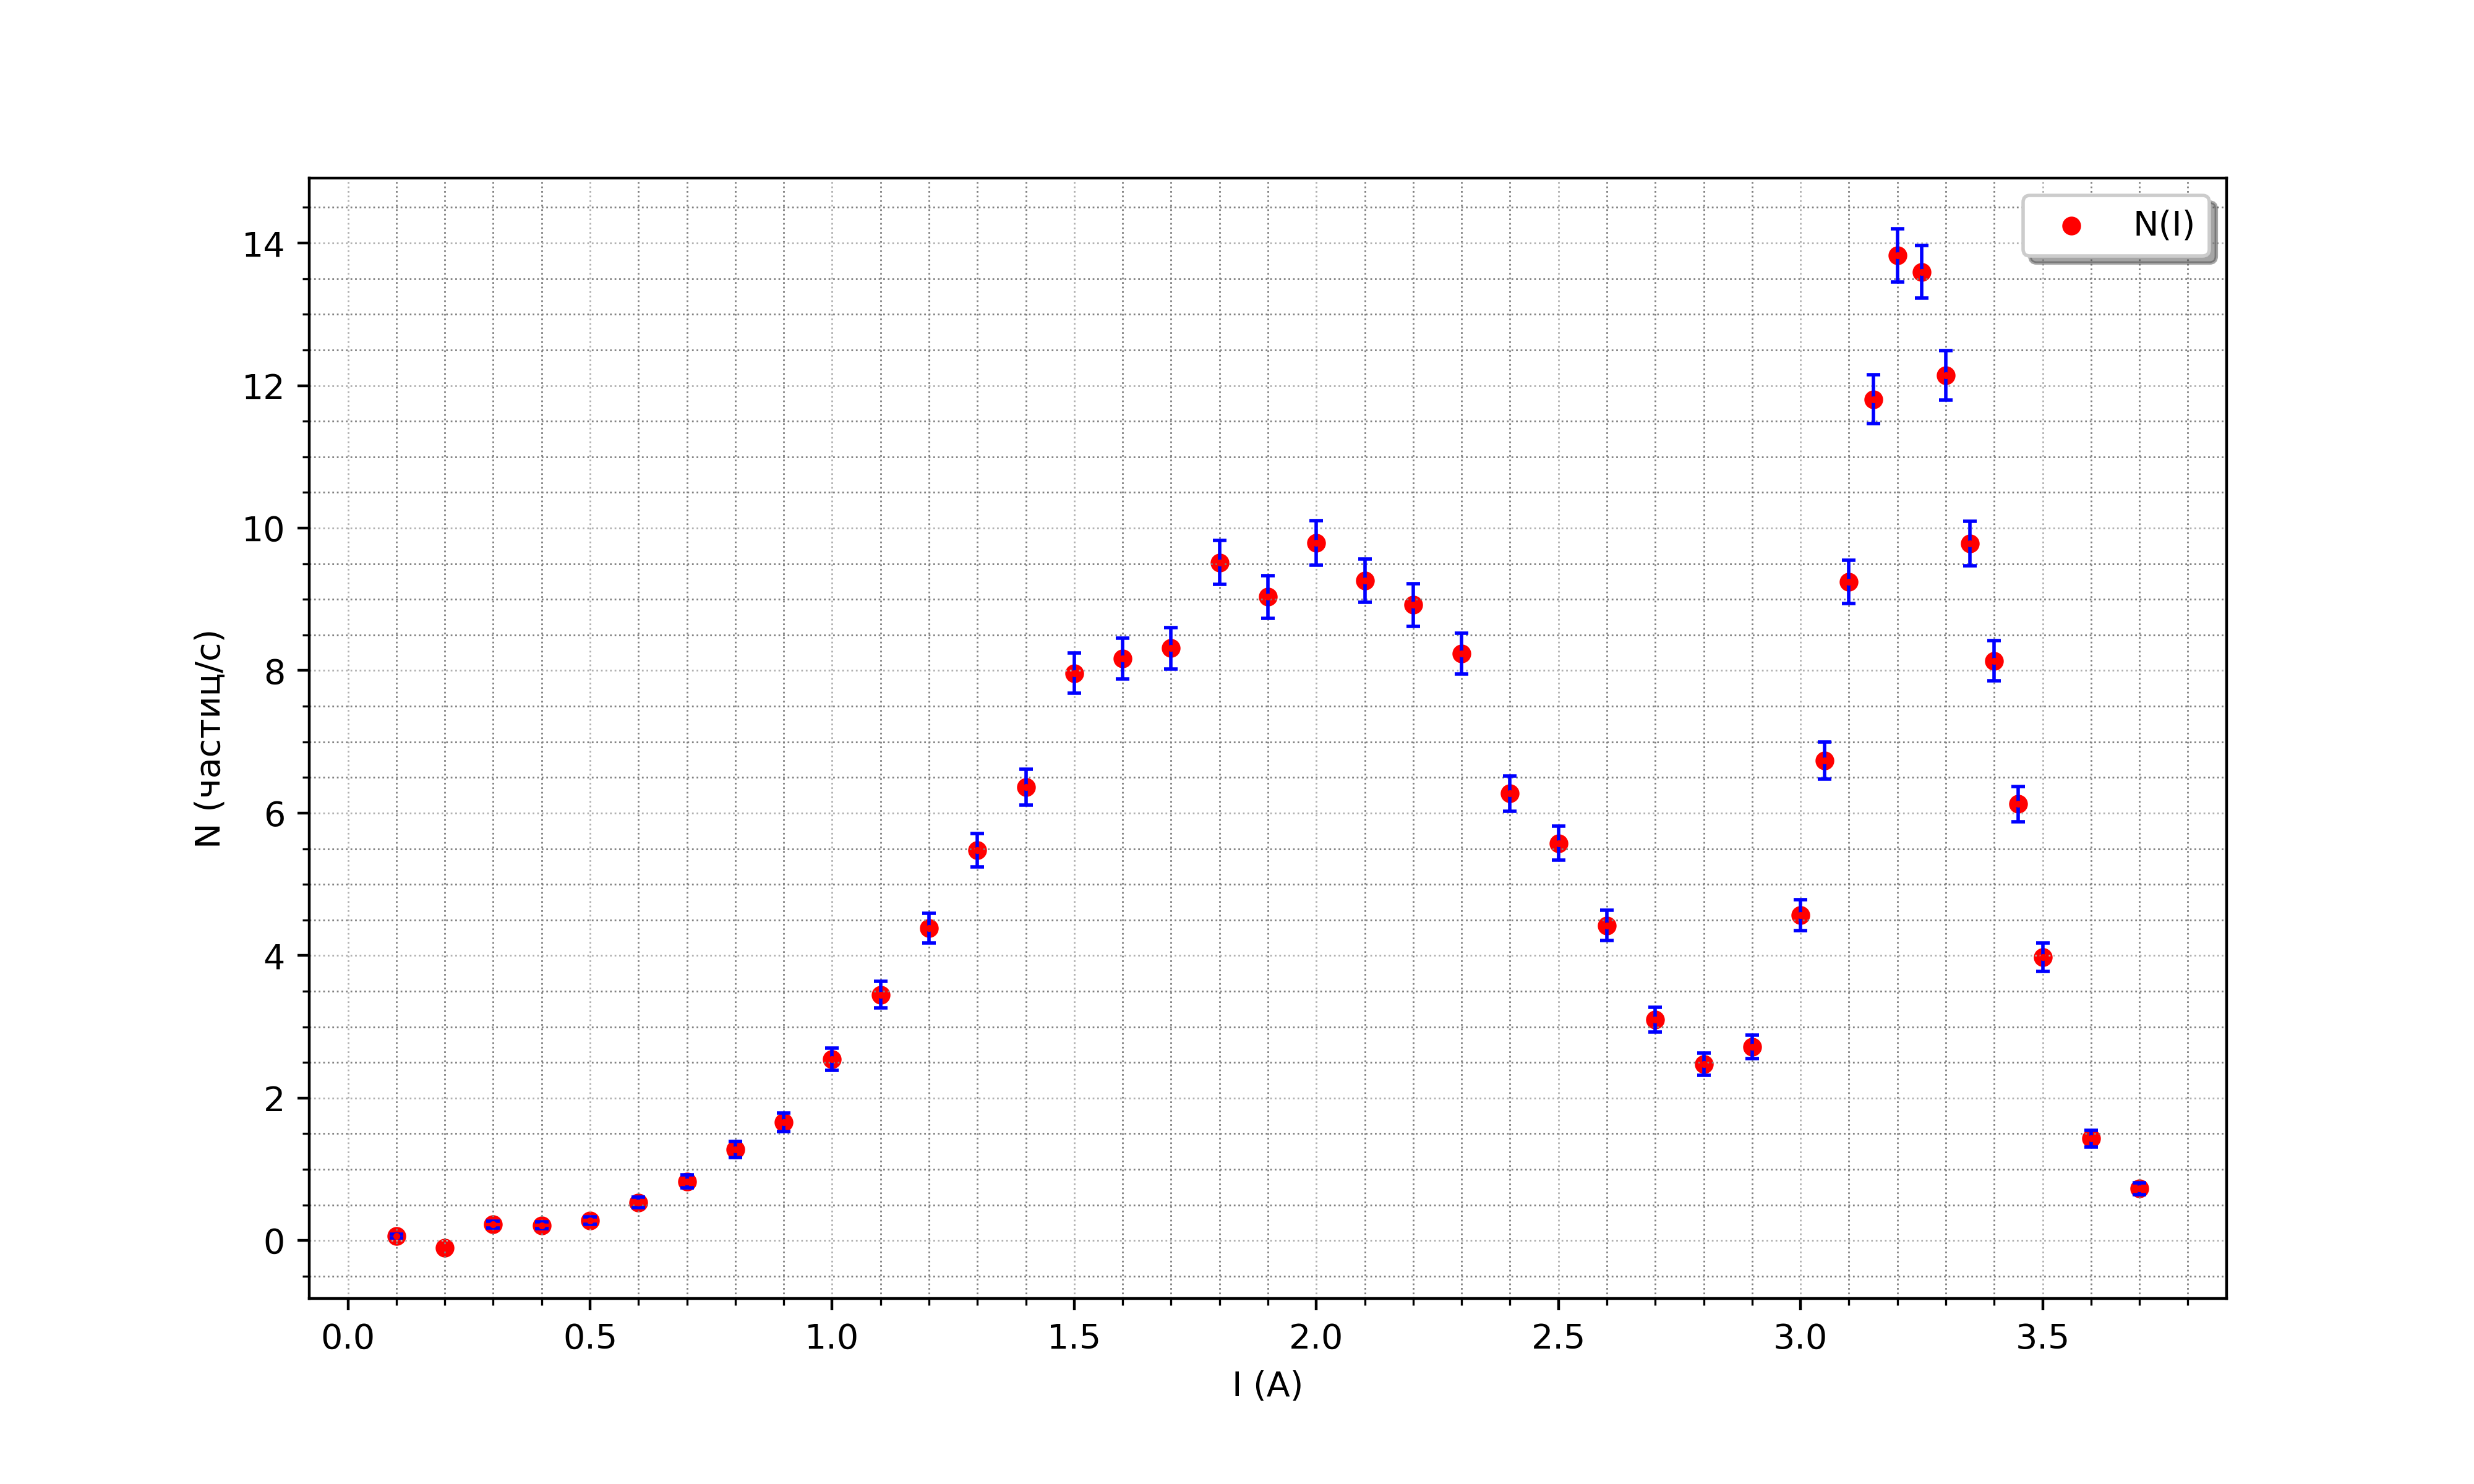
\includegraphics[scale = 0.54]{N(I).png}
        \caption{N(I)}
        \label{g1}
        \end{center}
    \end{figure}

    По значению $p_{\text{конв}}\cdot c = 1013,5$кэВ по формуле (\ref{eq7}) определим константу прибора
    $k \approx 316,7$

    Построим графики N(T) и $N(p_e)$

    \begin{figure}[h]
        \begin{center}
        \begin{minipage}[h]{0.47\linewidth}
        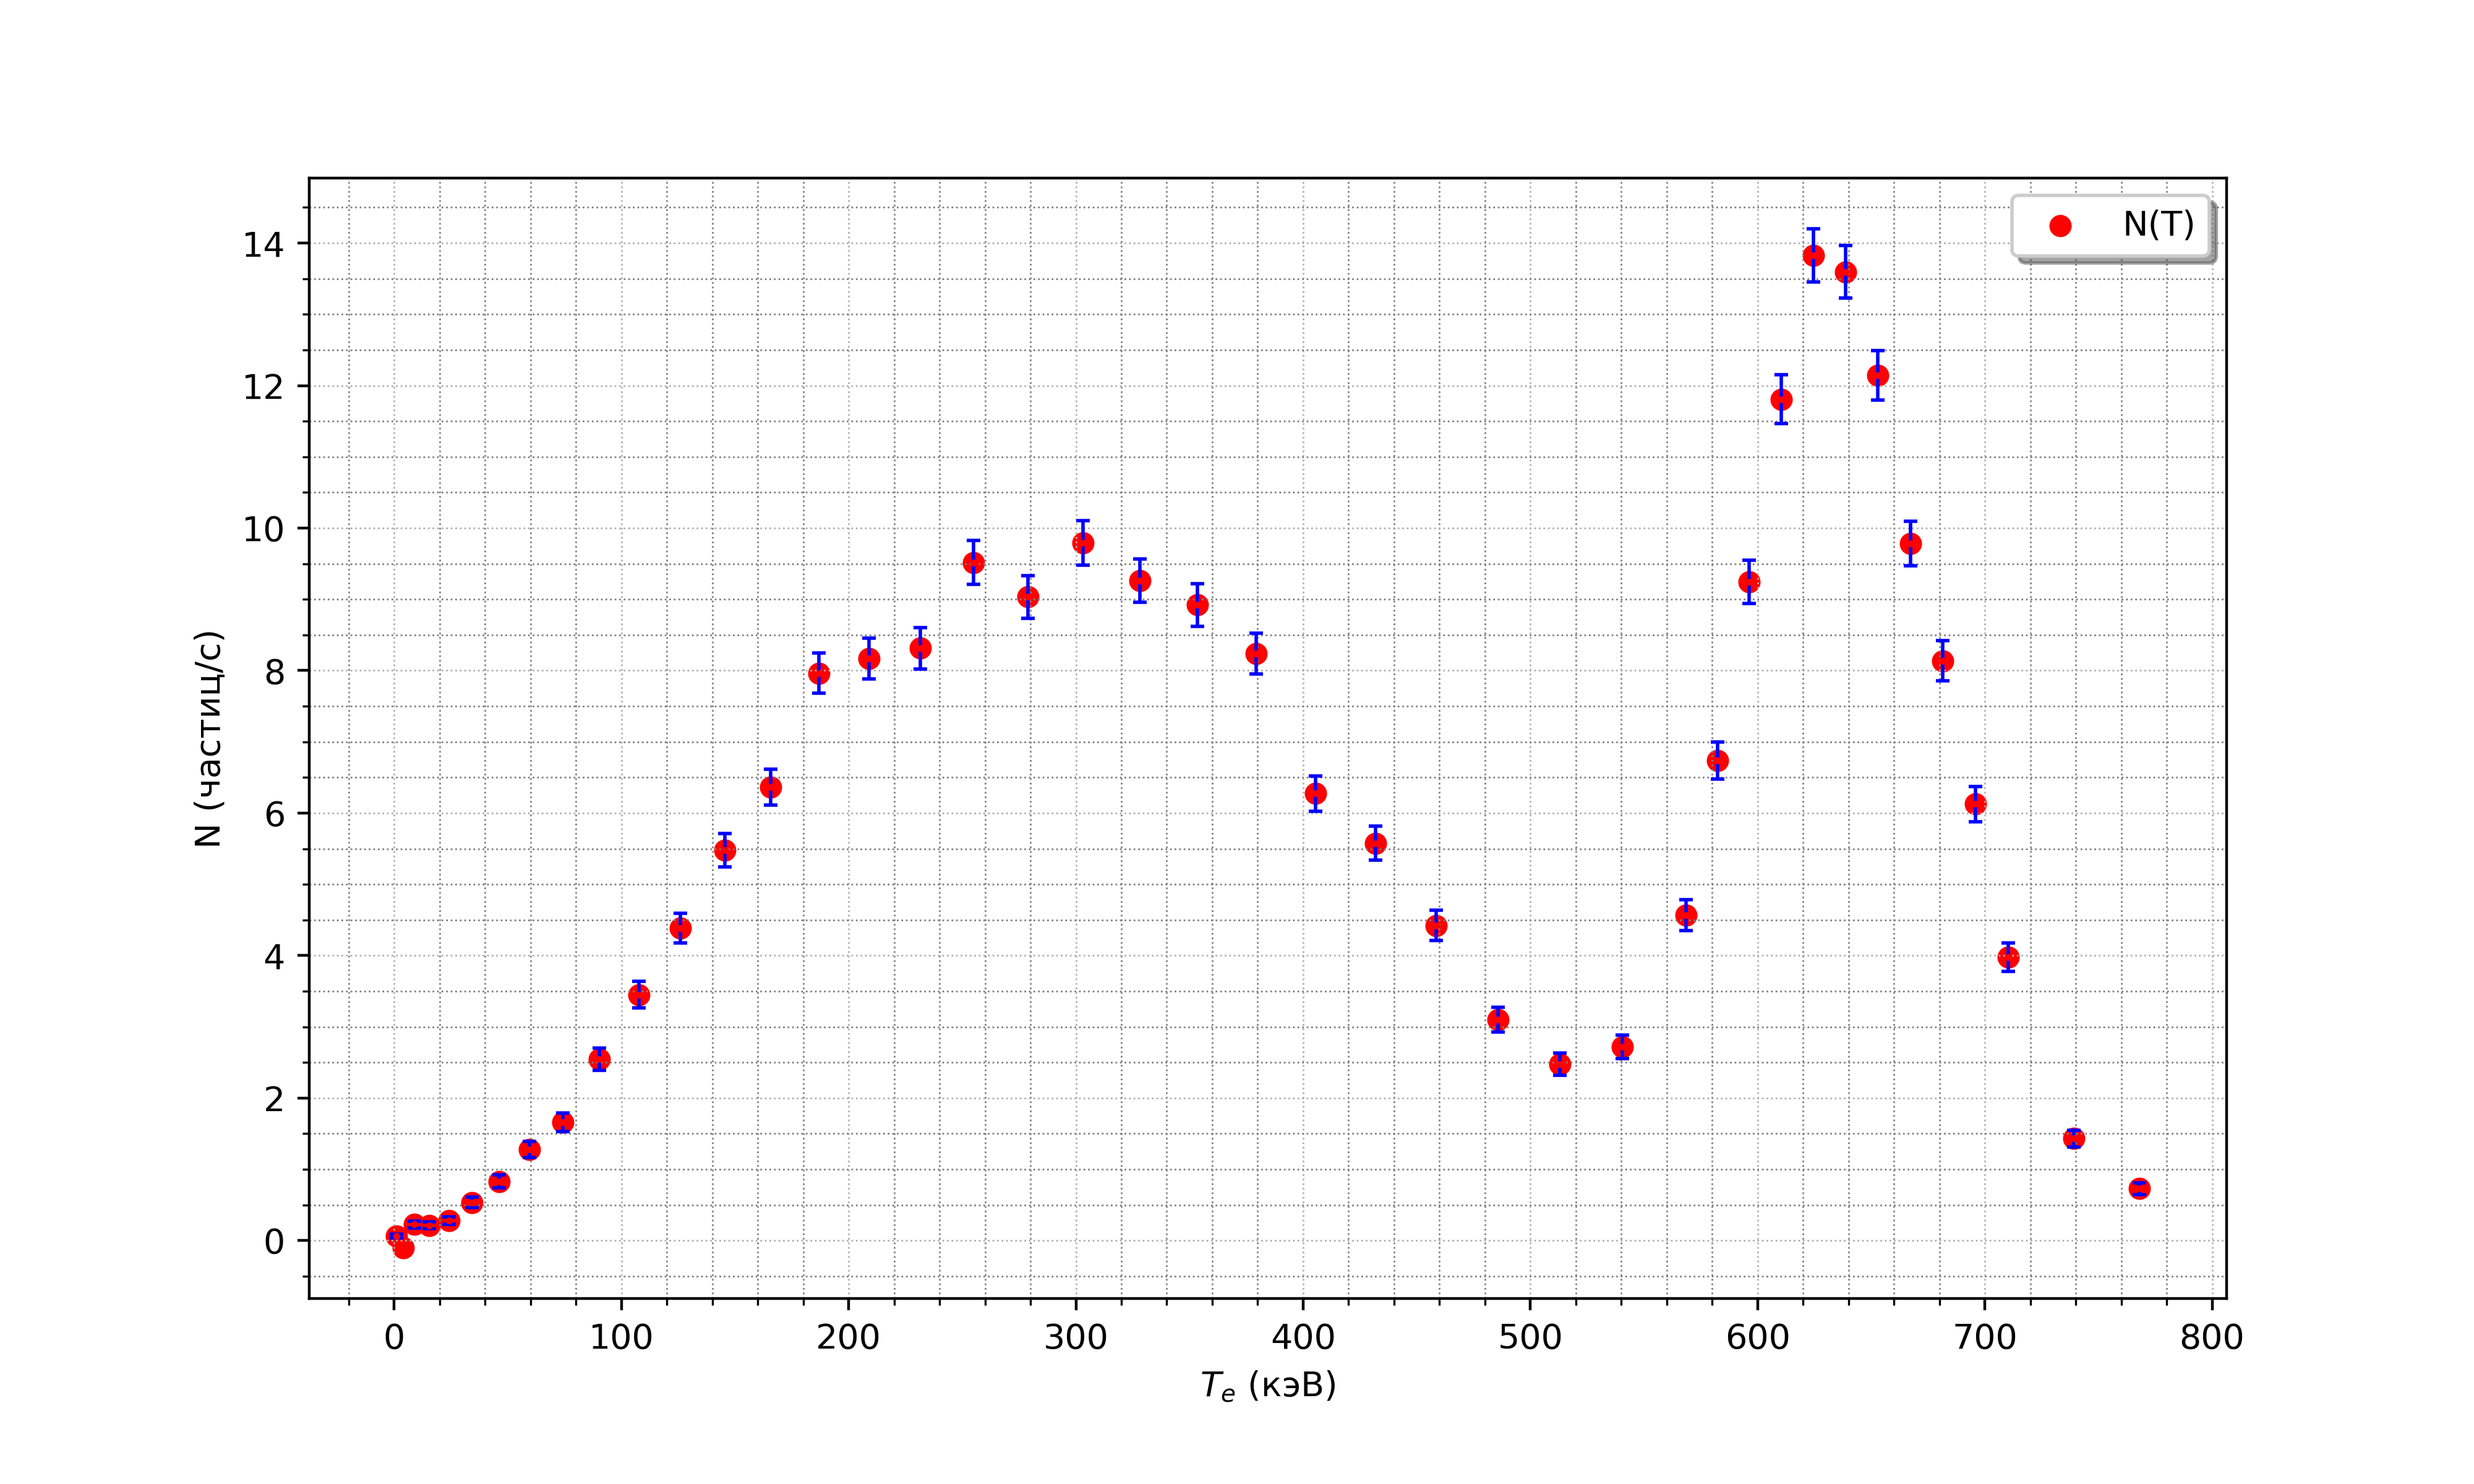
\includegraphics[width=1\linewidth]{N(T).png}
        \caption{} 
        \label{N(T)}
        \end{minipage}
        \hfill 
        \begin{minipage}[h]{0.47\linewidth}
        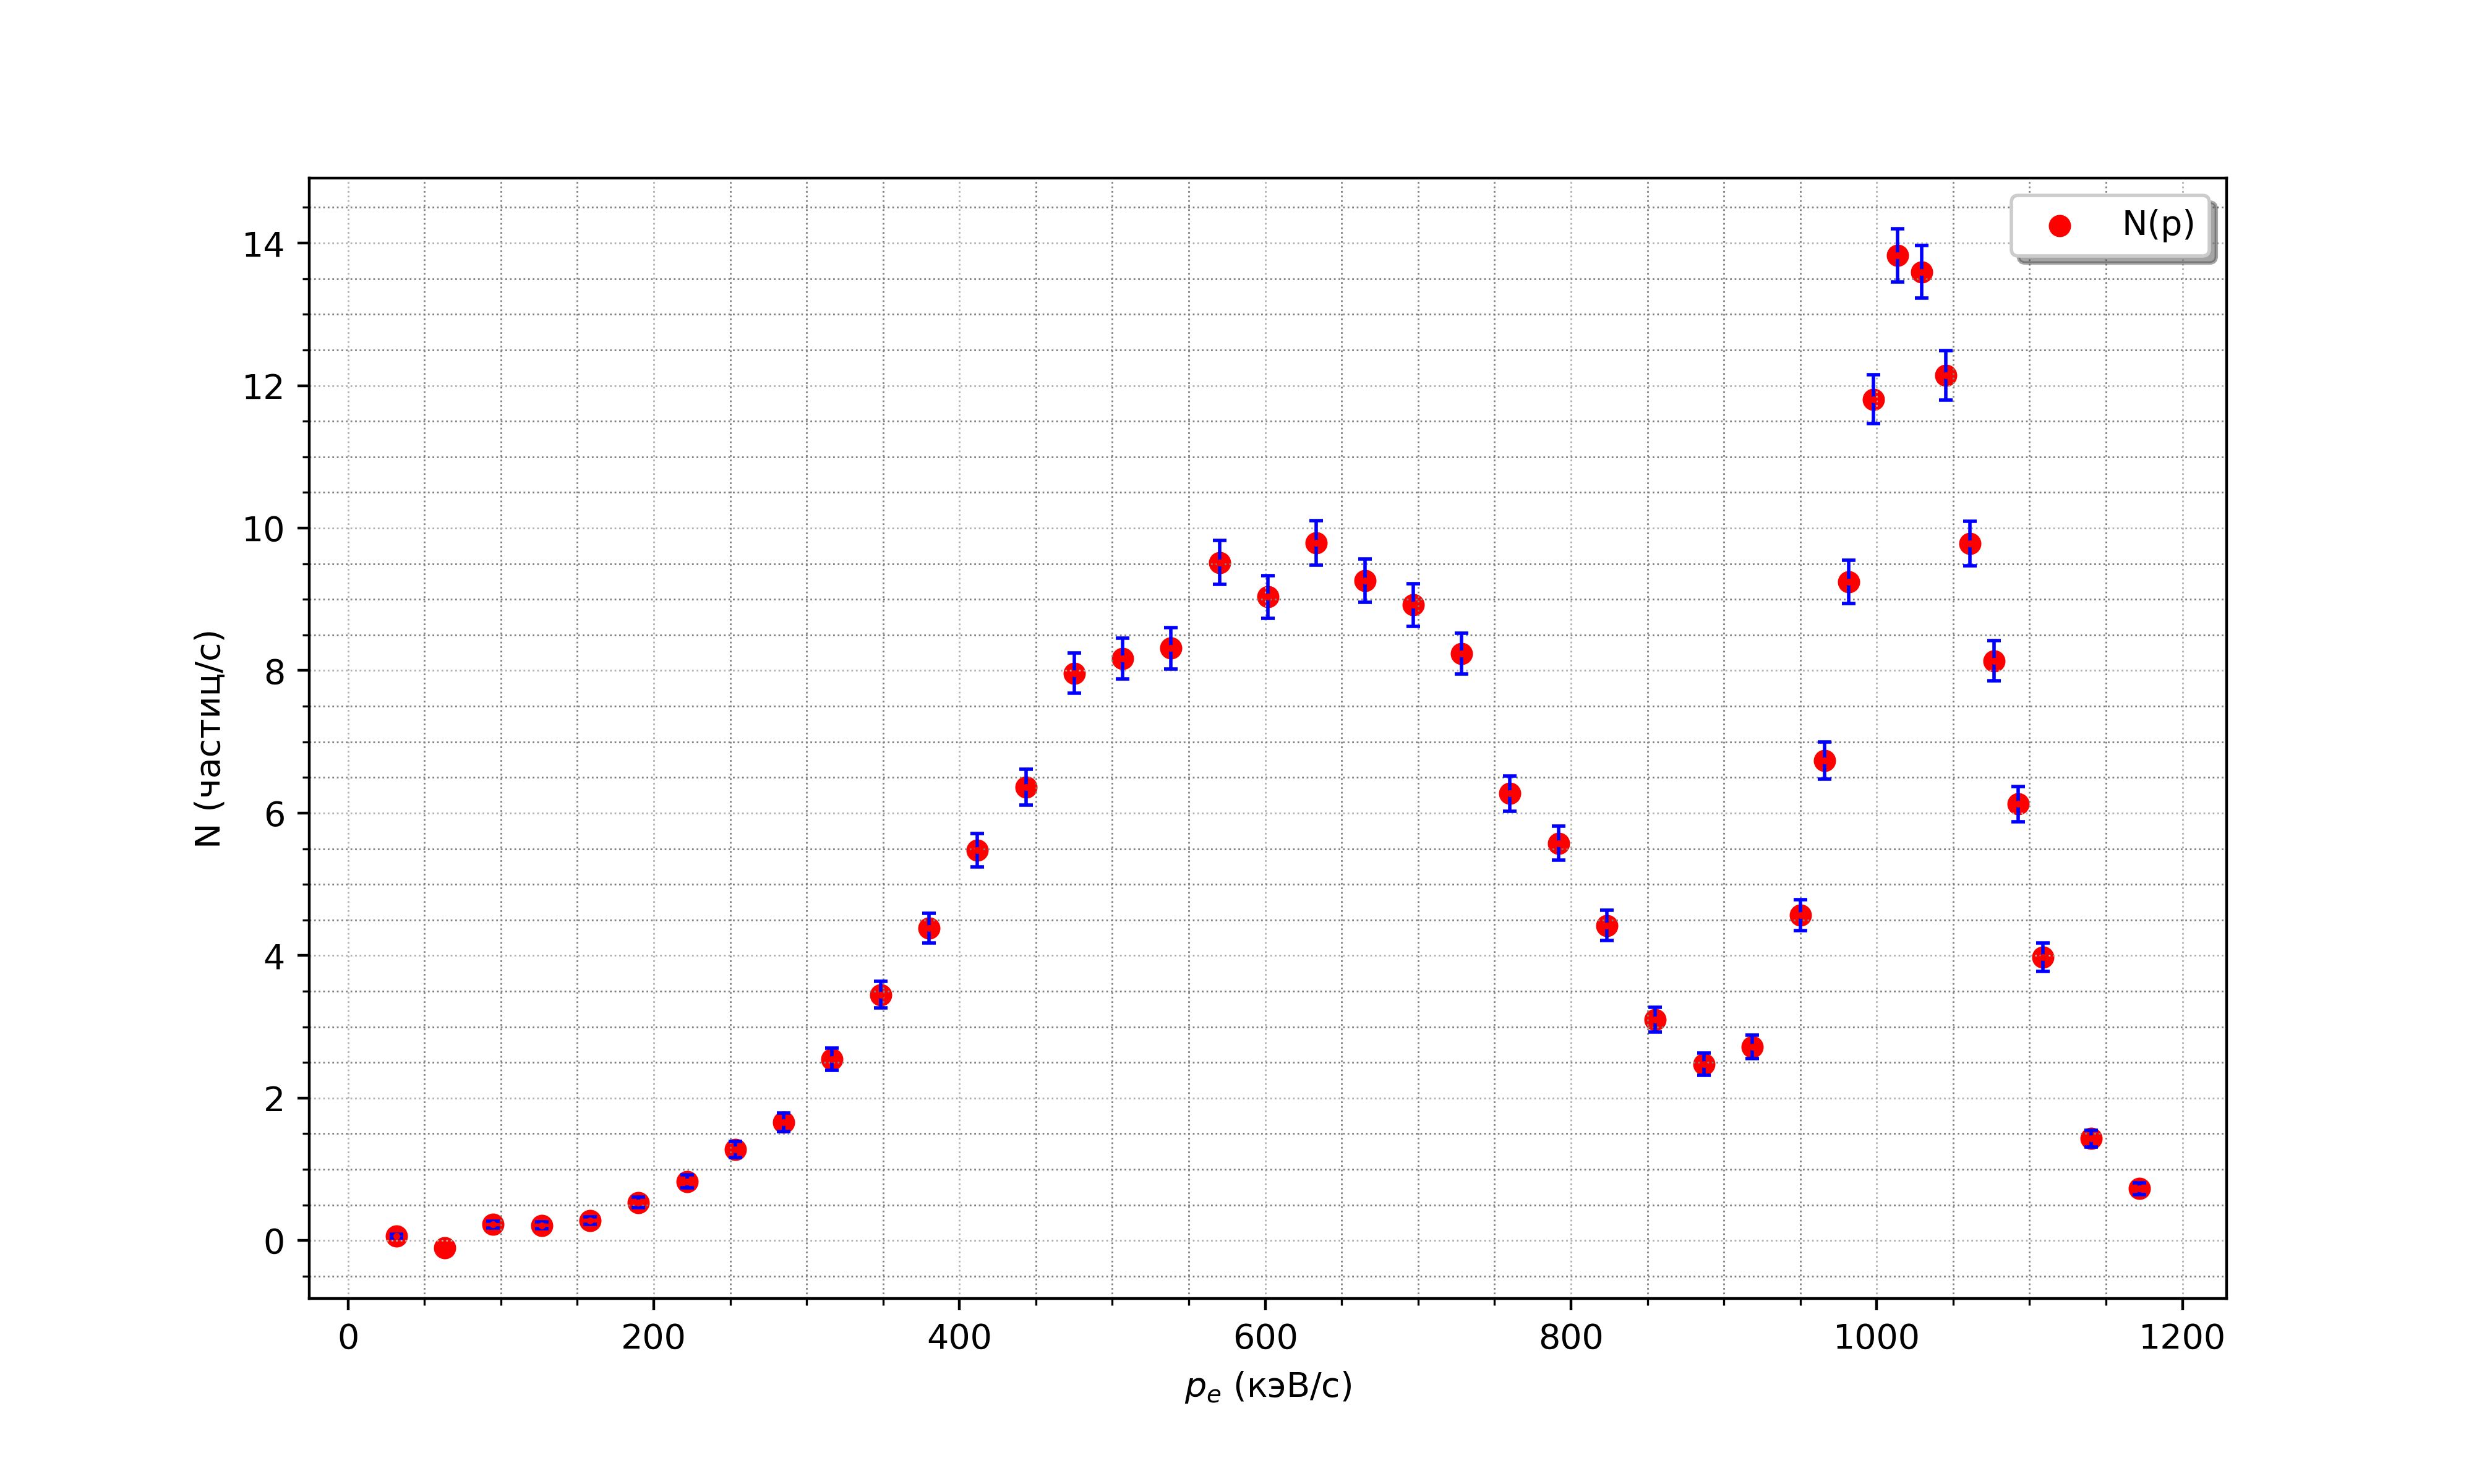
\includegraphics[width=1\linewidth]{N(p).png}
        \caption{}
        \label{N(p)}
        \end{minipage}
        \end{center}
    \end{figure}

    \item Определим $T_{max}$ с помощью графика Ферми. Подставим в (\ref{eq3}) значение $W(p_e)$
    из (\ref{eq10}) и разделим на $\Delta p_e$:

    \begin{equation}
        \sqrt{N(p_e)}\; / \; p^{3/2} \propto T_{max} - T
        \label{eq11}
    \end{equation}

    \begin{figure}[H]
        \begin{center}
        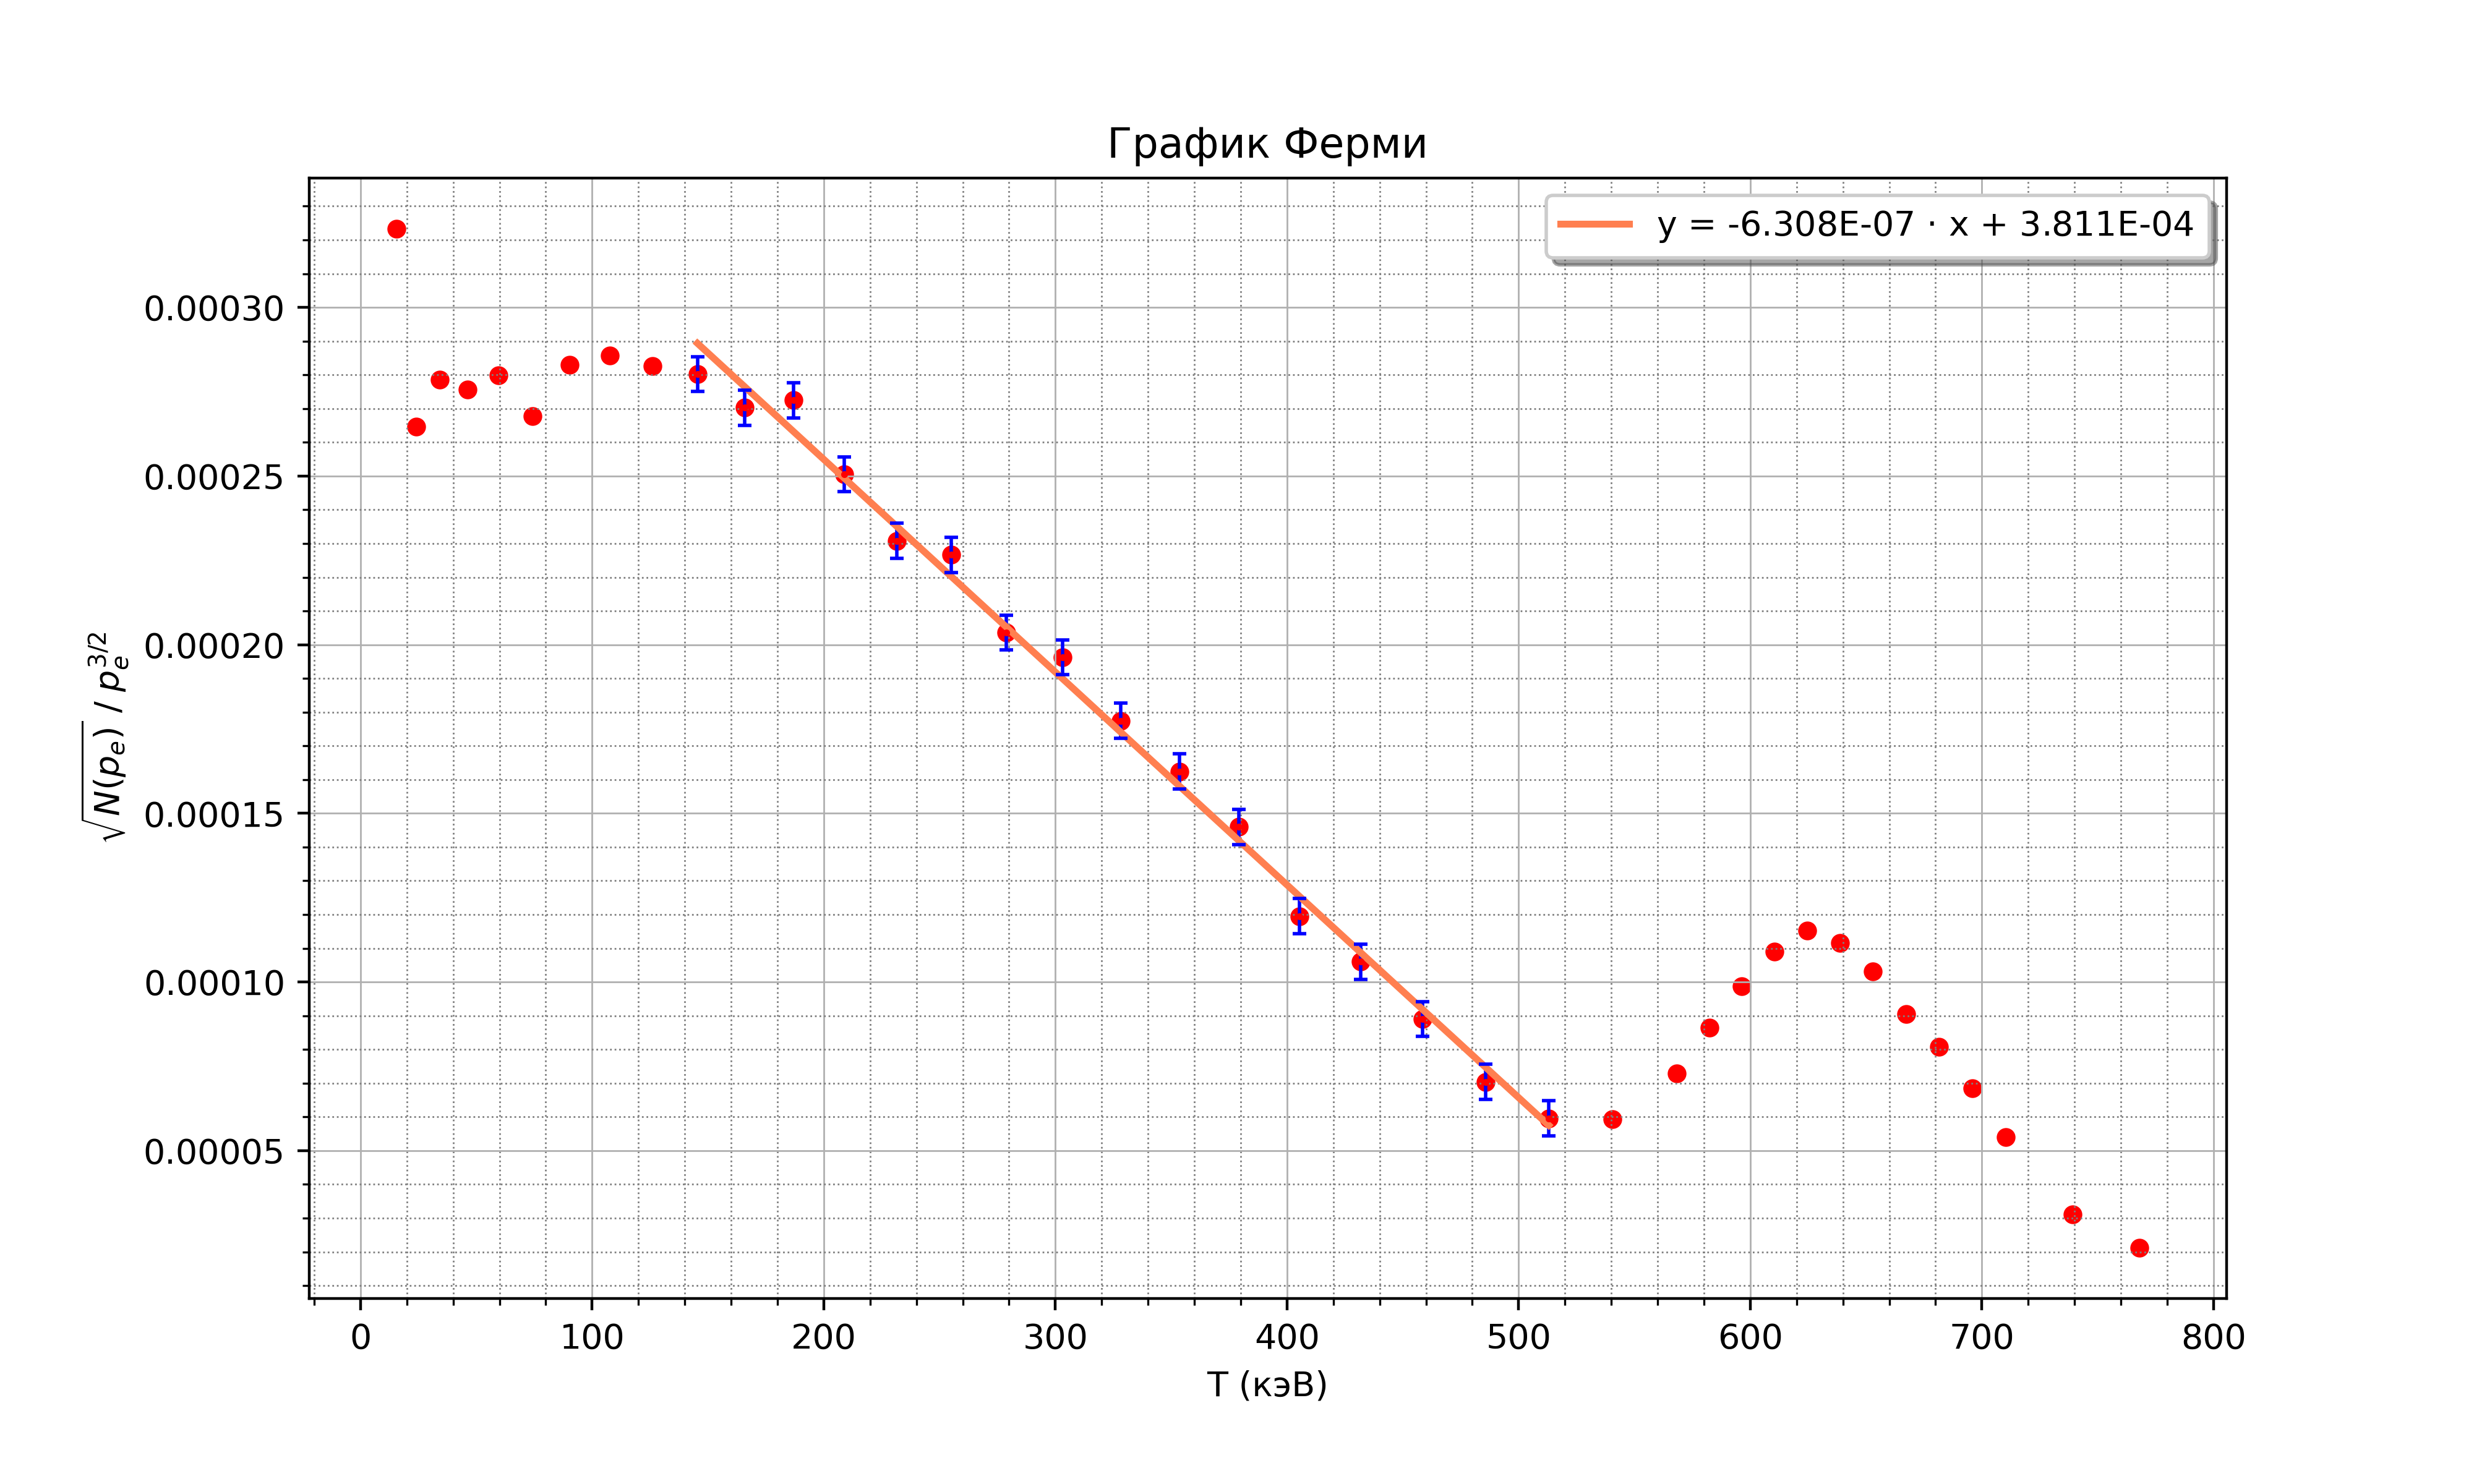
\includegraphics[scale = 0.7]{mkFermi.png}
        \caption{График Ферми}
        \label{g2}
        \end{center}
    \end{figure}

    По графику определим значение $T_{max} = 604.18 \pm 13.44\; \text{эВ} \;(2.22\%)$

\end{enumerate}

\section{Вывод}

В ходе работы было исследовано явление $\beta$-распада $^{137}Cs$. В спектр попали электроны, 
образованные в паре с антинейтрино при распаде, так же конверсионные электроны, испускаемые
возбужденными вторичными ядрами. С помощью графика Ферми $\sqrt{N(p_e)}\; / \; p^{3/2} \propto T_{max} - T$ 
было определено максимальное значение кинетической энергии $T_{max} = 604.18 \pm 13.44\; \text{эВ} \;(2.22\%)$.

\section{Литература}
Игошин Ф.Ф., Самарский Ю.А., Ципенюк Ю.М.  - Лабораторный практикум по общей физике: Учеб. пособие для вузов. Т. 3 Квантовая физика. 

\end{document}